\documentclass[a4paper, 12pt]{extarticle}
\usepackage[top=1in, bottom=1in, left=1in, right=1in]{geometry}
\usepackage{amsmath}
\usepackage{amssymb}
\usepackage{graphicx}
\usepackage{fontspec}
\usepackage{hyperref}
\usepackage{tikz}
\usepackage{fontspec}
%\usetikzlibrary{decorations.pathmorphing}
\usetikzlibrary{calc,decorations,patterns,arrows,decorations.pathmorphing,positioning}
\definecolor{pltblue}{HTML}{1F77B4}
\tikzset{every picture/.style={/utils/exec={\fontspec{Pretty Neat}}}}
\setmainfont{Pretty Neat}


\makeatletter
\pgfset{
  /pgf/decoration/randomness/.initial=2,
  /pgf/decoration/wavelength/.initial=100
}
\pgfdeclaredecoration{sketch}{init}{
  \state{init}[width=0pt,next state=draw,persistent precomputation={
    \pgfmathsetmacro\pgf@lib@dec@sketch@t0
  }]{}
  \state{draw}[width=\pgfdecorationsegmentlength,
  auto corner on length=\pgfdecorationsegmentlength,
  persistent precomputation={
    \pgfmathsetmacro\pgf@lib@dec@sketch@t{mod(\pgf@lib@dec@sketch@t+pow(\pgfkeysvalueof{/pgf/decoration/randomness},rand),\pgfkeysvalueof{/pgf/decoration/wavelength})}
  }]{
    \pgfmathparse{sin(2*\pgf@lib@dec@sketch@t*pi/\pgfkeysvalueof{/pgf/decoration/wavelength} r)}
    \pgfpathlineto{\pgfqpoint{\pgfdecorationsegmentlength}{\pgfmathresult\pgfdecorationsegmentamplitude}}
  }
  \state{final}{}
}
\tikzset{xkcd/.style={decorate,decoration={sketch,segment length=0.5pt,amplitude=0.5pt}}}
\makeatother

\usepackage{etoolbox}
\AtBeginEnvironment{tabular}{\fontspec{Pretty Neat}}

\setlength{\parindent}{0pt}
\setlength{\parskip}{0.5em}
\usepackage{fancyhdr}
\usepackage{geometry}
\usepackage{adjustbox}
\usepackage{titling}
\usepackage{multicol}
\usepackage{amsmath}
\usepackage{amssymb}
\usepackage{graphicx}
\usepackage{hyperref}
\usepackage{tikz}
\usepackage{fontspec}
\usetikzlibrary{calc,decorations,patterns,arrows,decorations.pathmorphing}
\definecolor{pltblue}{HTML}{1F77B4}

\usepackage{amsmath}
\usepackage{tikz}
\usepackage{enumitem}

\title{Random Walk Characteristics Worksheet}
\author{Network Science Course}
\date{}

\begin{document}

\section{Image Processing and Convolution}

\subsection{Preparation: Understanding Convolution}
Think of convolution as a way to find patterns in an image by looking through a small window (kernel). As we slide this window across the image, we:
\begin{enumerate}
    \item Look at a small neighborhood of pixels
    \item Multiply each pixel by the corresponding value in our pattern-matching window (kernel)
    \item Sum up these products to get a single number
    \item Move the window and repeat
\end{enumerate}

For example, if we want to detect vertical edges, we might use this kernel:
\[
K = \begin{bmatrix}
-1 & 1 & 0 \\
-1 & 1 & 0 \\
-1 & 1 & 0
\end{bmatrix}
\]

Let's see how it works on a small image region (3x3 pixels):

\[
\begin{bmatrix}
10 & 80 & 10 \\
10 & 80 & 10 \\
10 & 80 & 10
\end{bmatrix}
\]

We multiply each pixel by the corresponding kernel value and sum: $(10 \times -1 + 80 \times 1 + 10 \times 0) \times 3 = 210$. The high positive value (210) indicates a strong vertical edge was detected.
Here are some common kernel patterns:

\textbf{Vertical edge detection:}
\[
\begin{bmatrix}
-1 & 1 & 0 \\
-1 & 1 & 0 \\
-1 & 1 & 0
\end{bmatrix}
\quad
\text{Looks for } \xrightarrow{\text{dark to bright}}
\]

\textbf{Horizontal edge detection:}
\[
\begin{bmatrix}
-1 & -1 & -1 \\
1 & 1 & 1 \\
0 & 0 & 0
\end{bmatrix}
\quad
\text{Looks for } \downarrow \text{ dark to bright}
\]

\textbf{Blur/Smoothing:}
\[
\frac{1}{9}\begin{bmatrix}
1 & 1 & 1 \\
1 & 1 & 1 \\
1 & 1 & 1
\end{bmatrix}
\quad
\text{Averages all neighboring pixels}
\]

\clearpage

\subsection{Image Processing and Convolution}

Consider a 6x6 grayscale image showing a diagonal line pattern:

\begin{center}
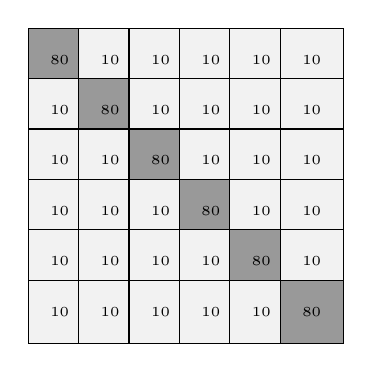
\begin{tikzpicture}[scale=0.8]
    % Create 6x6 grid
    \foreach \i in {0,...,5} {
        \foreach \j in {0,...,5} {
            \pgfmathsetmacro{\value}{ifthenelse(\i==\j, 80, 10)}
            \node[rectangle, draw, minimum size=0.8cm, fill=gray!\value] at (\i*0.8, -\j*0.8) {\tiny \value};
        }
    }
\end{tikzpicture}
\end{center}

\begin{enumerate}
\item If we want to detect diagonal edges, which kernel of size 3x3 would be most appropriate? The kernel should have the values between -1 and 1.
\begin{center}
    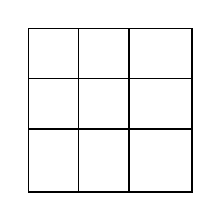
\begin{tikzpicture}[scale=0.8]
        % Create 6x6 grid
        \foreach \i in {0,...,2} {
            \foreach \j in {0,...,2} {
                \pgfmathsetmacro{\value}{ifthenelse(\i==\j, 10, 10)}
                \node[rectangle, draw, minimum size=0.8cm, fill=white] at (\i*0.8, -\j*0.8) {};
            }
        }
    \end{tikzpicture}
\end{center}

\item Apply your kernel to compute the convoluted image. No need to calculate the value of each pixel exactly but show your estimate by shading the pixels. For the boundary pixels, leave them blank since the kernel exceeds the boundary of the image.

\begin{center}
    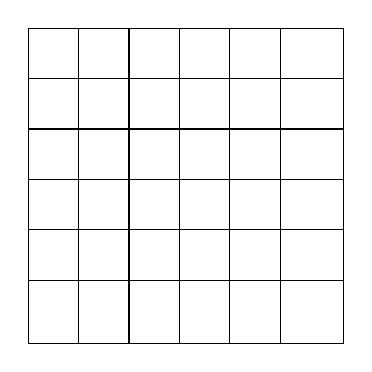
\begin{tikzpicture}[scale=0.8]
        % Create 6x6 grid
        \foreach \i in {0,...,5} {
            \foreach \j in {0,...,5} {
                \pgfmathsetmacro{\value}{ifthenelse(\i==\j, 80, 10)}
                \node[rectangle, draw, minimum size=0.8cm, fill=white] at (\i*0.8, -\j*0.8) {};
            }
        }
    \end{tikzpicture}
\end{center}

\item Now, let's learn how JPEG compression works. Consider this waves:

\begin{center}
    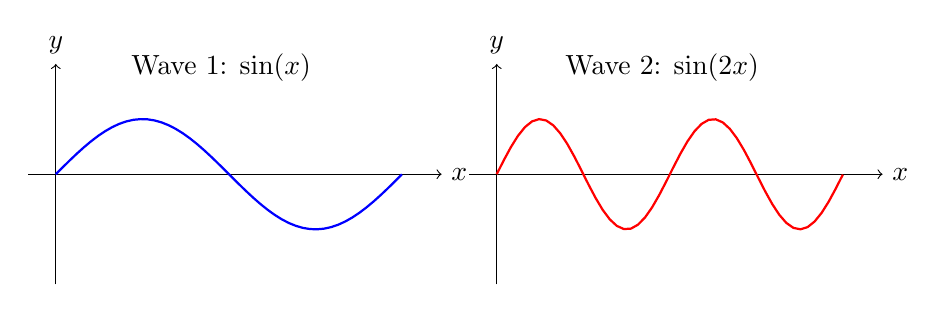
\begin{tikzpicture}[scale=0.7]
        % Wave 1
        \begin{scope}[xshift=0cm]
            \draw[->] (-0.5,0) -- (7,0) node[right] {$x$};
            \draw[->] (0,-2) -- (0,2) node[above] {$y$};
            \draw[thick, blue] plot[domain=0:6.28, samples=50] (\x, {sin(\x r)});
            \node[above] at (3,1.5) {Wave 1: $\sin(x)$};
        \end{scope}

        % Wave 2
        \begin{scope}[xshift=8cm]
            \draw[->] (-0.5,0) -- (7,0) node[right] {$x$};
            \draw[->] (0,-2) -- (0,2) node[above] {$y$};
            \draw[thick, red] plot[domain=0:6.28, samples=50] (\x, {sin(2*\x r)});
            \node[above] at (3,1.5) {Wave 2: $\sin(2x)$};
        \end{scope}
    \end{tikzpicture}
\end{center}

We combine these two waves by weighting the first wave by 1.5 and the second wave by 0.5. $\text{Combined Wave} = 1.5 \cdot \sin(x) + 0.5 \cdot \sin(2x)$. Draw the combined waves.

\begin{center}
\begin{tikzpicture}[scale=0.7]
    % Draw axes
    \draw[->] (-0.5,0) -- (7,0) node[right] {$x$};
    \draw[->] (0,-2) -- (0,2) node[above] {$y$};

    % Draw the composite wave
    %\draw[thick] plot[domain=0:6.28, samples=100]
    %    (\x, {1.5*sin(\x r) + 0.5*sin(2*\x r)});

    % Label
    \node[above] at (3,2) {Combined Wave};
\end{tikzpicture}
\end{center}

\item The Fourier transform is a reverse operation: it decomposes, not combines, waves into basic waves. The waves are continuous functions. But we can discretize them for computation as follows:

\begin{center}
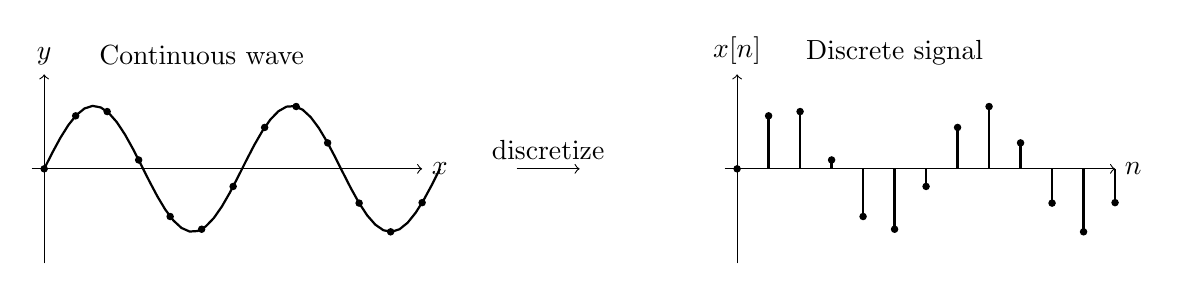
\begin{tikzpicture}[scale=0.8]
    % Original continuous wave
    \begin{scope}[xshift=-1cm]
        \draw[->] (-0.2,0) -- (6,0) node[right] {$x$};
        \draw[->] (0,-1.5) -- (0,1.5) node[above] {$y$};
        \draw[thick] plot[domain=0:2*pi, samples=50] (\x, {sin(2*\x r)});
        \node[above] at (2.5,1.5) {Continuous wave};

        % Draw sample points
        \foreach \x in {0,0.5,...,6} {
            \filldraw[black] (\x,{sin(2*\x r)}) circle (0.05);
        }
    \end{scope}

    % Arrow indicating discretization
    \draw[->] (6.5,0) -- (7.5,0);
    \node[above] at (7,0) {discretize};

    % Discretized signal
    \begin{scope}[xshift=10cm]
        \draw[->] (-0.2,0) -- (6,0) node[right] {$n$};
        \draw[->] (0,-1.5) -- (0,1.5) node[above] {$x[n]$};

        % Draw stems
        \foreach \x [count=\i from 0] in {0,0.5,...,6} {
            \draw[thick] (\i*0.5,0) -- (\i*0.5,{sin(2*\x r)});
            \filldraw[black] (\i*0.5,{sin(2*\x r)}) circle (0.05);
        }
        \node[above] at (2.5,1.5) {Discrete signal};
    \end{scope}
\end{tikzpicture}
\end{center}

This results in a vector of values $[10, 80, 10, 80, 10, 80, 10, 80]$. Now, let's create a discretized mixed wave $Z$ from $X$ and $Y$ as follows

\begin{align}
Z = X + Y = [10, 90, 30, 90, 10, 70, -10, 70, 10]
\end{align}
where
\begin{align}
X = [10, 80, 10, 80, 10, 80, 10, 80, 10], \quad
Y = [0, 10, 20, 10, 0, -10, -20, -10, 0]
\end{align}

(a) If we apply a kernel $K = [-1, 1, -1]$ to this signal, what will be the resulting signal? What kind of frequencies will this kernel emphasize?
\vspace{4em}

(c) If we apply a kernel $K = [1, 1, 1]$ to this signal, what will be the resulting signal? What kind of frequencies will this kernel emphasize?
\vspace{2em}

\clearpage

\item Just as 1D signals can be decomposed into sine waves, 2D images can be decomposed into 2D waves as follows. The Fourier transform can be applied to 2D images to decompose them into a sum of 2D waves.

\begin{center}
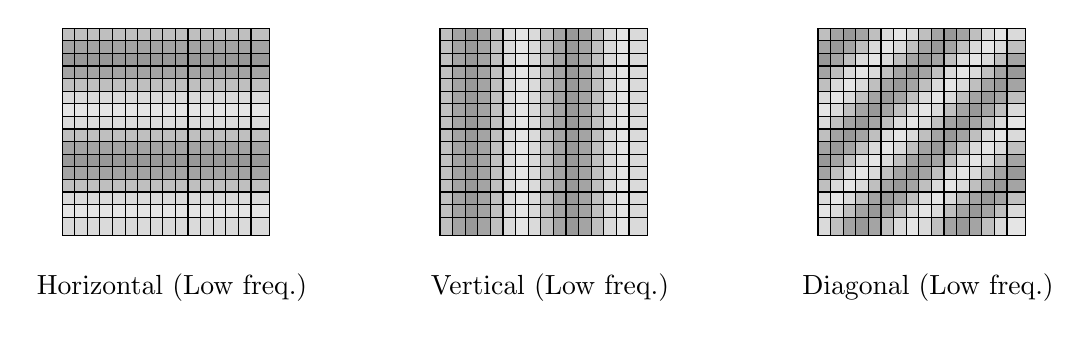
\begin{tikzpicture}[scale=0.8]
    % Horizontal wave (low frequency)
    \begin{scope}[xshift=0cm]
        \foreach \i in {0,...,15} {
            \foreach \j in {0,...,15} {
                \pgfmathsetmacro{\value}{50 + 30*sin(\j*45)}
                \node[rectangle, draw, minimum size=0.2cm, fill=gray!\value] at (\i*0.2, -\j*0.2) {};
            }
        }
        \node[below] at (1.6,-3.6) {Horizontal (Low freq.)};
    \end{scope}

    % Vertical wave
    \begin{scope}[xshift=6cm]
        \foreach \i in {0,...,15} {
            \foreach \j in {0,...,15} {
                \pgfmathsetmacro{\value}{50 + 30*sin(\i*45)}
                \node[rectangle, draw, minimum size=0.2cm, fill=gray!\value] at (\i*0.2, -\j*0.2) {};
            }
        }
        \node[below] at (1.6,-3.6) {Vertical (Low freq.)};
    \end{scope}

    % Diagonal wave
    \begin{scope}[xshift=12cm]
        \foreach \i in {0,...,15} {
            \foreach \j in {0,...,15} {
                \pgfmathsetmacro{\value}{50 + 30*sin((\i+\j)*45)}
                \node[rectangle, draw, minimum size=0.2cm, fill=gray!\value] at (\i*0.2, -\j*0.2) {};
            }
        }
        \node[below] at (1.6,-3.6) {Diagonal (Low freq.)};
    \end{scope}
\end{tikzpicture}

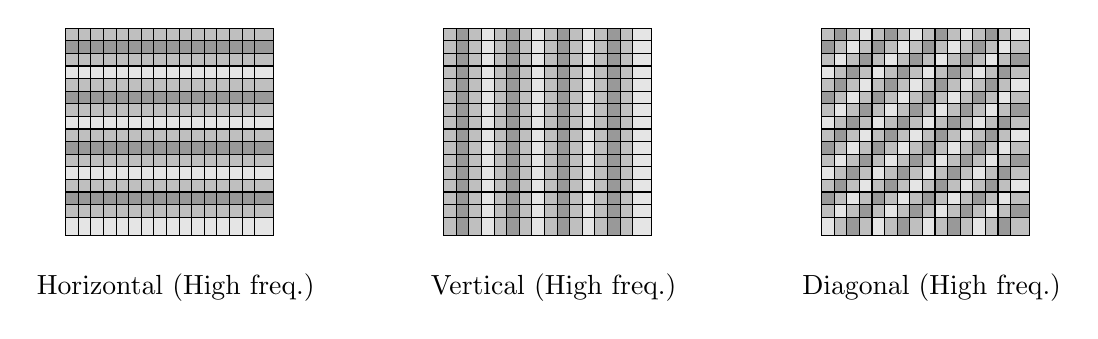
\begin{tikzpicture}[scale=0.8]
    % Horizontal wave (high frequency)
    \begin{scope}[xshift=0cm]
        \foreach \i in {0,...,15} {
            \foreach \j in {0,...,15} {
                \pgfmathsetmacro{\value}{50 + 30*sin(\j*90)}
                \node[rectangle, draw, minimum size=0.2cm, fill=gray!\value] at (\i*0.2, -\j*0.2) {};
            }
        }
        \node[below] at (1.6,-3.6) {Horizontal (High freq.)};
    \end{scope}

    % Vertical wave (high frequency)
    \begin{scope}[xshift=6cm]
        \foreach \i in {0,...,15} {
            \foreach \j in {0,...,15} {
                \pgfmathsetmacro{\value}{50 + 30*sin(\i*90)}
                \node[rectangle, draw, minimum size=0.2cm, fill=gray!\value] at (\i*0.2, -\j*0.2) {};
            }
        }
        \node[below] at (1.6,-3.6) {Vertical (High freq.)};
    \end{scope}

    % Diagonal wave (high frequency)
    \begin{scope}[xshift=12cm]
        \foreach \i in {0,...,15} {
            \foreach \j in {0,...,15} {
                \pgfmathsetmacro{\value}{50 + 30*sin((\i+\j)*90)}
                \node[rectangle, draw, minimum size=0.2cm, fill=gray!\value] at (\i*0.2, -\j*0.2) {};
            }
        }
        \node[below] at (1.6,-3.6) {Diagonal (High freq.)};
    \end{scope}
\end{tikzpicture}
\end{center}

Now, consider this checkerboard pattern on the left. Mark where you expect the highest magnitudes in the Fourier transform grid. The dashed circles represent the basis 2D waves in the Fourier domain.

\begin{center}
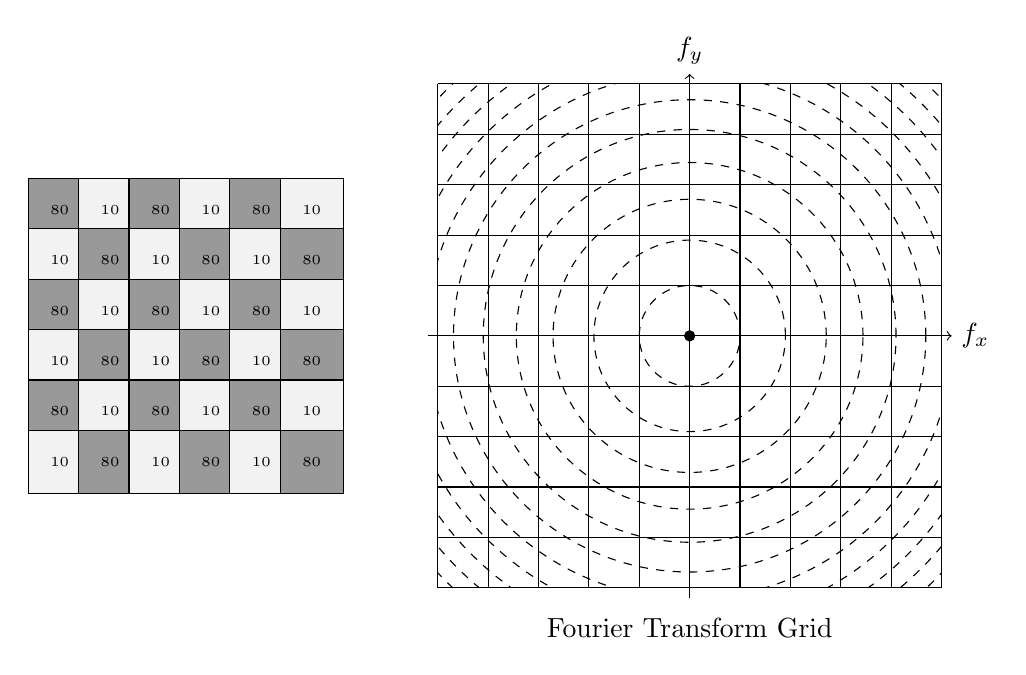
\begin{tikzpicture}[scale=0.8]
    % Create 6x6 checkerboard
    \begin{scope}[xshift=0cm, yshift=2cm]
    \foreach \i in {0,...,5} {
        \foreach \j in {0,...,5} {
            \pgfmathsetmacro{\value}{ifthenelse(mod(\i+\j,2)==0, 80, 10)}
            \node[rectangle, draw, minimum size=0.8cm, fill=gray!\value] at (\i*0.8, -\j*0.8) {\tiny \value};
        }
        }
    \end{scope}
    \begin{scope}[xshift=10cm,scale=0.8]
        % Draw main grid 7x7
        \draw (-5,-5) grid (5,5);

        % Draw coordinate axes
        \draw[->] (-5.2,0) -- (5.2,0) node[right] {$f_x$};
        \draw[->] (0,-5.2) -- (0,5.2) node[above] {$f_y$};

        % Add center dot
        \filldraw (0,0) circle (0.1);
        \node at (0,-5.8) {Fourier Transform Grid};

        % Add circles with radius up to 4.2 (to reach corners)
        % But clip them to show only within the grid
        \begin{scope}
            \clip (-5,-5) rectangle (5,5);
            \foreach \k in {1, ..., 40} {
                \pgfmathsetmacro{\r}{1 * (1 - 0.9^\k) / (1 - 0.9)}
                \draw[dashed] (0,0) circle (\r);
            }
        \end{scope}
    \end{scope}
\end{tikzpicture}
\end{center}

\item The image can be mapped to the Fourier transform grid (called frequency domain). We can also map it back to the original image domain (called spatial domain). Thus, we can manipulate the image in the frequency domain to remove some waves from the original image.
If we want to keep only the low-frequency components of the checkerboard pattern, what regions of the Fourier transform grid should we set to zero?

\end{enumerate}

\clearpage

\section{Color Spreading in Social Networks}
In a network of students forming study groups, each student starts with a preferred subject, shown by colors - Math (Blue), Physics (Green), or Arts (Red). Through their study group interactions, students influence each other's interests. The network diagram below shows students as circles connected by lines representing their study partnerships.

\begin{center}
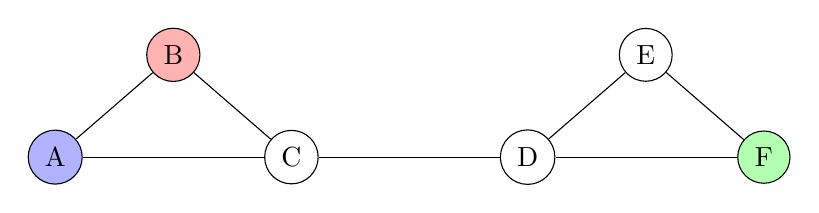
\begin{tikzpicture}[scale=1.5]
    % Nodes for first clique
    \node[circle,draw,fill=blue!30] (A) at (0,0) {A};
    \node[circle,draw,fill=red!30] (B) at (1,0.866) {B};
    \node[circle,draw,fill=white] (C) at (2,0) {C};

    % Nodes for second clique
    \node[circle,draw,fill=white] (D) at (4,0) {D};
    \node[circle,draw,fill=white] (E) at (5,0.866) {E};
    \node[circle,draw,fill=green!30] (F) at (6,0) {F};

    % Edges for first clique
    \draw (A) -- (B);
    \draw (B) -- (C);
    \draw (C) -- (A);

    % Edges for second clique
    \draw (D) -- (E);
    \draw (E) -- (F);
    \draw (F) -- (D);

    % Edge connecting the cliques
    \draw (C) -- (D);
\end{tikzpicture}
\end{center}

\begin{enumerate}[resume]

\item For each student, we'll follow this rule: "Adopt the most common subject among your study partners."
If tied, choose Math (Blue) > Arts (Red) > Physics (Green).
Now, let's start by looking at student D, who is currently undecided. What subject would student D choose?

\item Now look at student E. Using the same rule, what subject would they choose?

\item  Starting with nodes D, E, F, C, B, and A in that order, what color pattern emerges after many iterations?

\begin{center}
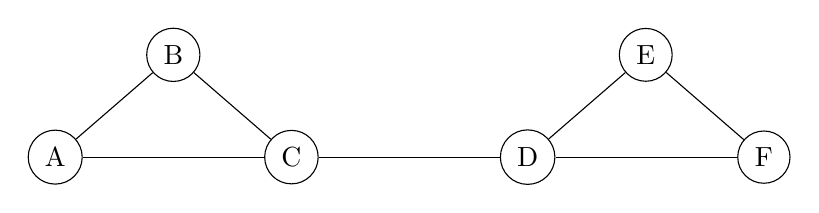
\begin{tikzpicture}[scale=1.5]
    % Nodes for first clique
    \node[circle,draw,fill=white] (A) at (0,0) {A};
    \node[circle,draw,fill=white] (B) at (1,0.866) {B};
    \node[circle,draw,fill=white] (C) at (2,0) {C};

    % Nodes for second clique
    \node[circle,draw,fill=white] (D) at (4,0) {D};
    \node[circle,draw,fill=white] (E) at (5,0.866) {E};
    \node[circle,draw,fill=white] (F) at (6,0) {F};

    % Edges for first clique
    \draw (A) -- (B);
    \draw (B) -- (C);
    \draw (C) -- (A);

    % Edges for second clique
    \draw (D) -- (E);
    \draw (E) -- (F);
    \draw (F) -- (D);

    % Edge connecting the cliques
    \draw (C) -- (D);
\end{tikzpicture}
\end{center}

\item If we repeat this process in order of A->B->C->D->E->F infinitely, what would be the final pattern of colors?

\begin{center}
    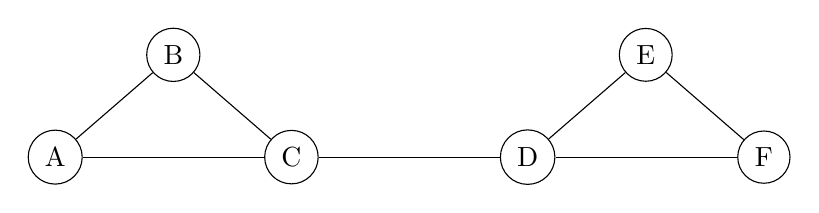
\begin{tikzpicture}[scale=1.5]
        % Nodes for first clique
        \node[circle,draw,fill=white] (A) at (0,0) {A};
        \node[circle,draw,fill=white] (B) at (1,0.866) {B};
        \node[circle,draw,fill=white] (C) at (2,0) {C};

        % Nodes for second clique
        \node[circle,draw,fill=white] (D) at (4,0) {D};
        \node[circle,draw,fill=white] (E) at (5,0.866) {E};
        \node[circle,draw,fill=white] (F) at (6,0) {F};

        % Edges for first clique
        \draw (A) -- (B);
        \draw (B) -- (C);
        \draw (C) -- (A);

        % Edges for second clique
        \draw (D) -- (E);
        \draw (E) -- (F);
        \draw (F) -- (D);

        % Edge connecting the cliques
        \draw (C) -- (D);
    \end{tikzpicture}
\end{center}

\item Let's introduce a self-reinforcing rule: When counting subjects among neighbors, a student's own chosen subject counts as an extra vote with weight three times as much as a vote from a neighbor. For example, if a student has chosen red and has two neighbors with green, red gets counted three times while green gets counted twice. Starting with nodes A, B, C, D, E, F in that order, what color pattern emerges after many iterations?

\begin{center}
    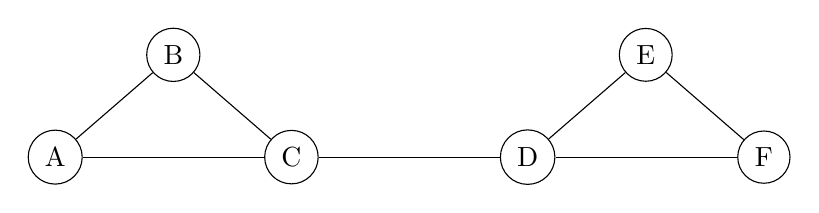
\begin{tikzpicture}[scale=1.5]
        % Nodes for first clique
        \node[circle,draw,fill=white] (A) at (0,0) {A};
        \node[circle,draw,fill=white] (B) at (1,0.866) {B};
        \node[circle,draw,fill=white] (C) at (2,0) {C};

        % Nodes for second clique
        \node[circle,draw,fill=white] (D) at (4,0) {D};
        \node[circle,draw,fill=white] (E) at (5,0.866) {E};
        \node[circle,draw,fill=white] (F) at (6,0) {F};

        % Edges for first clique
        \draw (A) -- (B);
        \draw (B) -- (C);
        \draw (C) -- (A);

        % Edges for second clique
        \draw (D) -- (E);
        \draw (E) -- (F);
        \draw (F) -- (D);

        % Edge connecting the cliques
        \draw (C) -- (D);
    \end{tikzpicture}
\end{center}

\end{enumerate}

\clearpage

\begin{enumerate}[resume]

\item Let's make it more operational. Each color can be represented as a one-hot vector as follows:
\begin{multicols}{2}
\begin{itemize}
    \item Blue (Math) = [1,0,0]
    \item Green (Science) = [0,1,0]
\end{itemize}
\columnbreak
\begin{itemize}
    \item Red (Arts) = [0,0,1]
    \item White (Undecided) = [0,0,0]
\end{itemize}
\end{multicols}

Then, how can we represent the rule "Adopt the most common subject among your study partners" as a computational operation? Ignore self-reinforcing rule. Hint: it is a max-pooling operation.


\vspace{10em}
\item Design a computational operation that follows the self-reinforcing rule without altering the operation in the previous question?

\vspace{10em}
\item What if we use ``mean'' instead of ``max'' and repeat the operation infinitely? Draw the final pattern of colors. There is no tie in this case.

\begin{center}
    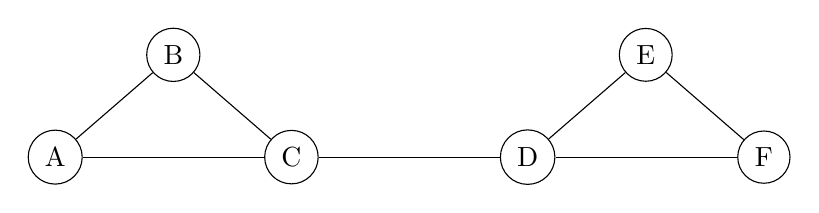
\begin{tikzpicture}[scale=1.5]
        % Nodes for first clique
        \node[circle,draw,fill=white] (A) at (0,0) {A};
        \node[circle,draw,fill=white] (B) at (1,0.866) {B};
        \node[circle,draw,fill=white] (C) at (2,0) {C};

        % Nodes for second clique
        \node[circle,draw,fill=white] (D) at (4,0) {D};
        \node[circle,draw,fill=white] (E) at (5,0.866) {E};
        \node[circle,draw,fill=white] (F) at (6,0) {F};

        % Edges for first clique
        \draw (A) -- (B);
        \draw (B) -- (C);
        \draw (C) -- (A);

        % Edges for second clique
        \draw (D) -- (E);
        \draw (E) -- (F);
        \draw (F) -- (D);

        % Edge connecting the cliques
        \draw (C) -- (D);
    \end{tikzpicture}
\end{center}

\item What if we use ``sum'' operation and repeat the operation infinitely?
\end{enumerate}

\clearpage

\section{The Weisfeiler-Lehman Test}
The color spreading process we just studied is closely related to a fundamental concept in graph theory called the Weisfeiler-Lehman (WL) test. This test helps us determine if two graphs might be structurally different by looking at how colors spread through them.

\begin{enumerate}[resume]
\item Consider these two graphs. Are they the same (isomorphic)?

\begin{center}
\begin{tikzpicture}[scale=1.5]
    % First graph
    \begin{scope}[xshift=0cm]
        \node[circle,draw,fill=blue!30] (A1) at (0,0) {1};
        \node[circle,draw,fill=red!30] (B1) at (1,0) {2};
        \node[circle,draw,fill=green!30] (C1) at (0.5,0.866) {3};
        \node[circle,draw,fill=yellow!30] (D1) at (0.5,-0.866) {4};

        \draw[xkcd] (A1) -- (B1);
        \draw[xkcd] (B1) -- (C1);
        \draw[xkcd] (C1) -- (A1);
        \draw[xkcd] (A1) -- (D1);
        \draw[xkcd] (B1) -- (D1);
    \end{scope}

    % Second graph
    \begin{scope}[xshift=4cm]
        \node[circle,draw,fill=blue!30] (A2) at (0,0) {a};
        \node[circle,draw,fill=red!30] (B2) at (1,0) {b};
        \node[circle,draw,fill=green!30] (C2) at (0.5,0.866) {c};
        \node[circle,draw,fill=yellow!30] (D2) at (0.5,-0.866) {d};

        \draw[xkcd] (A2) -- (B2);
        \draw[xkcd] (B2) -- (C2);
        \draw[xkcd] (C2) -- (A2);
        \draw[xkcd] (A2) -- (D2);
        \draw[xkcd] (C2) -- (D2);
    \end{scope}
\end{tikzpicture}
\end{center}

\item Now let's look at how the WL test works:
\begin{itemize}
    \item For each node,
    \begin{itemize}
        \item Collect the colors of its neighbors (including itself)
        \item Count the frequency of each color, and create a list of color frequencies in order of Red, Green, Blue. For example, if there are two reds, one green, and one blue, the sorted frequency list is [2, 1, 1].
    \end{itemize}
    \item Once all nodes have been processed, reassign the same color to the nodes with the same sorted frequency list.
    \item Count the number of nodes for each color, and create a sorted list of color frequencies for a graph.
\end{itemize}

For the graphs above, perform one iteration of the WL test, and provide the colors of the nodes after the iteration, and the sorted color frequency list for each graph.


\begin{center}
    \begin{tikzpicture}[scale=1.5]
        % First graph
        \begin{scope}[xshift=0cm]
            \node[circle,draw,fill=white] (A1) at (0,0) {1};
            \node[circle,draw,fill=white] (B1) at (1,0) {2};
            \node[circle,draw,fill=white] (C1) at (0.5,0.866) {3};
            \node[circle,draw,fill=white] (D1) at (0.5,-0.866) {4};

            \draw[xkcd] (A1) -- (B1);
            \draw[xkcd] (B1) -- (C1);
            \draw[xkcd] (C1) -- (A1);
            \draw[xkcd] (A1) -- (D1);
            \draw[xkcd] (B1) -- (D1);
        \end{scope}

        % Second graph
        \begin{scope}[xshift=4cm]
            \node[circle,draw,fill=white] (A2) at (0,0) {a};
            \node[circle,draw,fill=white] (B2) at (1,0) {b};
            \node[circle,draw,fill=white] (C2) at (0.5,0.866) {c};
            \node[circle,draw,fill=white] (D2) at (0.5,-0.866) {d};

            \draw[xkcd] (A2) -- (B2);
            \draw[xkcd] (B2) -- (C2);
            \draw[xkcd] (C2) -- (A2);
            \draw[xkcd] (A2) -- (D2);
            \draw[xkcd] (C2) -- (D2);
        \end{scope}

    \end{tikzpicture}
    \end{center}

    Sorted color frequency list (the first graph): \underline{\hspace{5cm}} \\

    \vspace{1em}

    Sorted color frequency list (the second graph): \underline{\hspace{5cm}}


\vspace{2em}

\item Consider these two graphs. At first glance, they look similar. Apply one iteration of the WL test to see if they're actually the same:
\begin{center}
    \begin{tikzpicture}[scale=1.5]
        % First graph
        \begin{scope}[xshift=0cm]
            \node[circle,draw,fill=white] (n1) at (0,0) {1};
            \node[circle,draw,fill=white] (n2) at (1,0) {2};
            \node[circle,draw,fill=white] (n3) at (0,1) {3};
            \node[circle,draw,fill=white] (n4) at (1,1) {4};
            \node[circle,draw,fill=white] (n5) at (2,0.) {5};
            \node[circle,draw,fill=white] (n6) at (3,0.5) {6};

            \draw[xkcd] (n1) -- (n2);
            \draw[xkcd] (n1) -- (n3);
            \draw[xkcd] (n2) -- (n4);
            \draw[xkcd] (n3) -- (n4);
            \draw[xkcd] (n4) -- (n5);
            \draw[xkcd] (n5) -- (n6);
            \draw[xkcd] (n4) -- (n6);
        \end{scope}

        % Second graph with very different layout
                % Second graph with very different layout
                \begin{scope}[xshift=4cm]
                    \node[circle,draw,fill=white] (m1) at (0.8,1.2) {A};
                    \node[circle,draw,fill=white] (m2) at (0,0.6) {B};
                    \node[circle,draw,fill=white] (m3) at (1.6,0.6) {C};
                    \node[circle,draw,fill=white] (m4) at (0.8,0) {D};
                    \node[circle,draw,fill=white] (m5) at (0,-0.6) {E};
                    \node[circle,draw,fill=white] (m6) at (1.6,-0.6) {F};

                    \draw[xkcd] (m1) -- (m2);
                    \draw[xkcd] (m1) -- (m3);
                    \draw[xkcd] (m2) -- (m4);
                    \draw[xkcd] (m3) -- (m4);
                    \draw[xkcd] (m4) -- (m5);
                    \draw[xkcd] (m5) -- (m6);
                    \draw[xkcd] (m4) -- (m6);
                \end{scope}
    \end{tikzpicture}
    \end{center}

\item Apply one iteration of the WL test to the two graphs above. And then apply the second iteration. Provide the colors of the nodes after the iteration, and the sorted color frequency list for each graph.

First iteration:
\begin{center}
    \begin{tikzpicture}[scale=1.5]
        % First graph
        \begin{scope}[xshift=0cm]
            \node[circle,draw,fill=white] (n1) at (0,0) {1};
            \node[circle,draw,fill=white] (n2) at (1,0) {2};
            \node[circle,draw,fill=white] (n3) at (0,1) {3};
            \node[circle,draw,fill=white] (n4) at (1,1) {4};
            \node[circle,draw,fill=white] (n5) at (2,0.) {5};
            \node[circle,draw,fill=white] (n6) at (3,0.5) {6};

            \draw[xkcd] (n1) -- (n2);
            \draw[xkcd] (n1) -- (n3);
            \draw[xkcd] (n2) -- (n4);
            \draw[xkcd] (n3) -- (n4);
            \draw[xkcd] (n4) -- (n5);
            \draw[xkcd] (n5) -- (n6);
            \draw[xkcd] (n4) -- (n6);
        \end{scope}

        % Second graph with very different layout
                % Second graph with very different layout
                \begin{scope}[xshift=4cm]
                    \node[circle,draw,fill=white] (m1) at (0.8,1.2) {A};
                    \node[circle,draw,fill=white] (m2) at (0,0.6) {B};
                    \node[circle,draw,fill=white] (m3) at (1.6,0.6) {C};
                    \node[circle,draw,fill=white] (m4) at (0.8,0) {D};
                    \node[circle,draw,fill=white] (m5) at (0,-0.6) {E};
                    \node[circle,draw,fill=white] (m6) at (1.6,-0.6) {F};

                    \draw[xkcd] (m1) -- (m2);
                    \draw[xkcd] (m1) -- (m3);
                    \draw[xkcd] (m2) -- (m4);
                    \draw[xkcd] (m3) -- (m4);
                    \draw[xkcd] (m4) -- (m5);
                    \draw[xkcd] (m5) -- (m6);
                    \draw[xkcd] (m4) -- (m6);
                \end{scope}
    \end{tikzpicture}
    \end{center}

Second iteration:
\begin{center}
    \begin{tikzpicture}[scale=1.5]
        % First graph
        \begin{scope}[xshift=0cm]
            \node[circle,draw,fill=white] (n1) at (0,0) {1};
            \node[circle,draw,fill=white] (n2) at (1,0) {2};
            \node[circle,draw,fill=white] (n3) at (0,1) {3};
            \node[circle,draw,fill=white] (n4) at (1,1) {4};
            \node[circle,draw,fill=white] (n5) at (2,0.) {5};
            \node[circle,draw,fill=white] (n6) at (3,0.5) {6};

            \draw[xkcd] (n1) -- (n2);
            \draw[xkcd] (n1) -- (n3);
            \draw[xkcd] (n2) -- (n4);
            \draw[xkcd] (n3) -- (n4);
            \draw[xkcd] (n4) -- (n5);
            \draw[xkcd] (n5) -- (n6);
            \draw[xkcd] (n4) -- (n6);
        \end{scope}

        % Second graph with very different layout
                % Second graph with very different layout
                \begin{scope}[xshift=4cm]
                    \node[circle,draw,fill=white] (m1) at (0.8,1.2) {A};
                    \node[circle,draw,fill=white] (m2) at (0,0.6) {B};
                    \node[circle,draw,fill=white] (m3) at (1.6,0.6) {C};
                    \node[circle,draw,fill=white] (m4) at (0.8,0) {D};
                    \node[circle,draw,fill=white] (m5) at (0,-0.6) {E};
                    \node[circle,draw,fill=white] (m6) at (1.6,-0.6) {F};

                    \draw[xkcd] (m1) -- (m2);
                    \draw[xkcd] (m1) -- (m3);
                    \draw[xkcd] (m2) -- (m4);
                    \draw[xkcd] (m3) -- (m4);
                    \draw[xkcd] (m4) -- (m5);
                    \draw[xkcd] (m5) -- (m6);
                    \draw[xkcd] (m4) -- (m6);
                \end{scope}
    \end{tikzpicture}
    \end{center}

\item The WL test is heuristic and not always correct. Consider a graph of six nodes forming a ring. Create another non-isomorphic graph with the same number of nodes, and edges that the WL test results in the same color frequency list.

\begin{flushleft}
    \begin{tikzpicture}[scale=1.2]
        % Nodes in a regular hexagon
        \node[circle,draw,fill=white] (n1) at (0:1) {1};
        \node[circle,draw,fill=white] (n2) at (60:1) {2};
        \node[circle,draw,fill=white] (n3) at (120:1) {3};
        \node[circle,draw,fill=white] (n4) at (180:1) {4};
        \node[circle,draw,fill=white] (n5) at (240:1) {5};
        \node[circle,draw,fill=white] (n6) at (300:1) {6};

        % Edges forming the ring
        \draw[xkcd] (n1) -- (n2);
        \draw[xkcd] (n2) -- (n3);
        \draw[xkcd] (n3) -- (n4);
        \draw[xkcd] (n4) -- (n5);
        \draw[xkcd] (n5) -- (n6);
        \draw[xkcd] (n6) -- (n1);
    \end{tikzpicture}
\end{flushleft}


\item What is the difference between the WL test and the color spreading process we studied in the previous section?

\end{enumerate}
\end{document}

\end{document}